% !TeX root = ../libro.tex
% !TeX encoding = utf8

\setchapterpreamble[c][0.75\linewidth]{%
	\sffamily
	Una vez hemos construido un algoritmo correcto, un paso importante es determinar su costo computacional, es decir, los recursos que necesita, tales como el tiempo o espacio. El análisis necesario para estimar estos costes es un problema teórico, para el cuál requeriremos de un marco formal, que definiremos al principio de este capítulo. \\
	Además veremos los costes de los algoritmos estudiados en el \autoref{ch:tercer-capitulo}.
	\par\bigskip
}
\chapter{Complejidad algorítmica}\label{ch:cuarto-capitulo}


Como ya mencionamos anteriormente, necesitamos un marco formal para estudiar la complejidad de un algoritmo, por ello utilizaremos la notación asintótica, que introducimos con las siguientes definiciones.

\begin{definicion}
	Dadas dos funciones $f,g:\mathbb{N}\rightarrow \mathbb{R}$ diremos que $f(n)=\Theta(g(n))$ si existen constantes $c_1,c_2$ y $n_0$ tales que $$0\leq c_1g(n)\leq f(n)\leq c_2g(n)\ \ \ \forall n\geq n_0.$$
\end{definicion}

\begin{definicion}
	Dadas dos funciones $f,g:\mathbb{N}\rightarrow \mathbb{R}$ diremos que $f(n)=O(g(n))$ si existen constantes $c$ y $n_0$ tales que $$0\leq f(n)\leq cg(n)\ \ \ \forall n\geq n_0.$$
\end{definicion}

\begin{definicion}
	Dadas dos funciones $f,g:\mathbb{N}\rightarrow \mathbb{R}$ diremos que $f(n)=\Omega(g(n))$ si existen constantes $c$ y $n_0$ tales que $$0\leq cg(n)\leq f(n)\ \ \ \forall n\geq n_0.$$
\end{definicion}

En esencia, la idea es establecer una cota para el crecimiento asintótico de una función a partir de otra, normalmente más simple. En particular, la notación $\Omega$ implica una cota inferior, $O$ una cota superior y $\Theta$ ambas. En la \autoref{fig:notacion_asintotica} podemos observar un ejemplo de cada tipo de notación. \\

Utilizaremos la notación asintótica principalmente para describir el tiempo de ejecución de los algoritmos, pues es el recurso más importante, normalmente. \\

Cuando hablamos de tiempo de ejecución, hay que especificar de qué tiempo estamos hablando exactamente, pues existen varios interesantes. Entre otros, el tiempo medio de ejecución, el del peor caso, o el del mejor. Normalmente los datos más interesantes son el tiempo medio, pues es el tiempo de ejecución medio del algoritmo, y el tiempo de ejecución del peor caso, que establece un límite al tiempo de ejecución del algoritmo.

\begin{figure}[!htb]
	\centering
	\begin{subfigure}{\linewidth}
		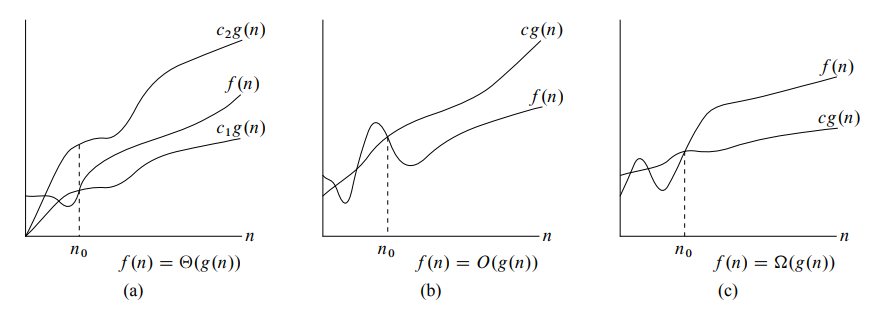
\includegraphics[width=14cm]{notacion_asintotica}
	\end{subfigure}
	
	\caption{Ejemplos gráficos de las notaciones $\Theta,O$ y $\Omega$. En cada imagen se muestra el valor mínimo para $n_0$, pero cualquier valor superior funciona también. Para el caso \textbf{(a)}, la notación $\Theta(g(n))$ implica una cota superior e inferior, por lo que la gráfica de $f(n)$ debe situarse entre las cotas obtenidas a partir de $g(n)$ y las constantes $c_1$ y $c_2$. En \textbf{(b)}, la notación $O(g(n))$ establece una cota superior, por lo que la gráfica de $f(n)$ se debe situar por debajo de la cota, obtenida a partir de la constante $c$. Por último, en \textbf{(c)} la notación $\Omega$ implica una cota inferior, luego en este caso, la gráfica de $f(n)$ debe de estar por encima de dicha cota, obtenida a partir de $c$. La imagen ha sido extraída de la referencia \cite{algorithms}, capítulo 3, figura 3.1.}
	\label{fig:notacion_asintotica}
\end{figure}


\endinput



